\documentclass[8pt,landscape]{article}
\usepackage{multicol}
\usepackage{amsmath}
\usepackage{amssymb}
\usepackage{amsthm}
\usepackage{commath}
\usepackage[landscape]{geometry}
\usepackage{enumitem}
\usepackage{graphicx}
\usepackage{mdframed}
\usepackage{tikz}
\usepackage{mathrsfs}
\usepackage{titlesec}
\titleformat*{\section}{\small\bfseries}
\titleformat*{\subsection}{\footnotesize\bfseries}

\geometry{top=0.5in,bottom=0.5in,left=0.5in,right=0.5in}

\begin{document}
	\small 
	\begin{multicols*}{4}
		\section*{1. Speaking Mathematically}
		\begin{itemize}[leftmargin=*]
			\item variable: place holder for an object
			\item statement: sentence that is true or false, but not both
		\end{itemize}
		\section*{2. Logic of compound statements}
		\begin{itemize}[leftmargin=*]
			\item $p\rightarrow q \equiv \neg p \lor q$
			\item converse: $ q\rightarrow p$
			\item inverse: $\neg p \rightarrow \neg q$
			\item order of operations for logical operators: 1) negations, 2) $\land, \lor$, 3) $\longrightarrow, \longleftrightarrow$
			\item sufficient condition: r is a sufficient condition for s means ``if r then s"
			\item necessary condition: r is a necessary condition for s means ``if not r then not s"
			\item r is a necessary and sufficient condition for s: ``r if, and only if, s"
		\end{itemize}
		\subsection*{Valid Argument Forms}
		\begin{itemize}[leftmargin=*]
			\item modus ponens: $p\rightarrow q;p;q.$
			\item modus tollens: $p\rightarrow q;\neg q;p.$
			\item generalization: $p;p\lor q$ and mirror
			\item specialization: $p\land q;p.$ and mirror
			\item elimination: $p\lor q;\neg q;p.$ and mirror
			\item transitivity: $p\rightarrow q;q\rightarrow r;r.$
		\end{itemize}

		\section*{3. Logic of Quantified Statements}
		\begin{itemize}[leftmargin=*]
			\item Predicate: a sentence with finitely many variables that becomes a statement when each variable is concretely instantiated.
			\item Domain of a predicate variable (i.e. a variable in a predicate) is the set of all values it can hold
			\item Truth Set of $P(x)$ where $x$ has domain $D$ is $\{x \in D \mid P(x)\}$
			\end{itemize}
		\section*{4. Elementary Number Theory \& Methods of Proof}
		\subsection*{4.1 to 4.3}
		for integers $n>1:$
		\begin{itemize}[leftmargin=*]
		\item $n$ is prime $\Leftrightarrow \forall r,s \in\mathbb{Z^{+}}, n=rs \rightarrow (r=1 \land s=n) \lor (r=n \land s=1)$
		\item $n$ is composite $\Leftrightarrow \exists r,s \in\mathbb{Z^{+}}$ s.t. $1<r<n \land 1<s<n \land rs=n$
		\end{itemize}
		\textbf{Divisibility:} (for $n,d \in\mathbb{Z}, d\neq0$) $d\mid n \Leftrightarrow \exists k\in\mathbb{Z}, n=dk$
		\subsection*{4.4 to 4.6}
		\begin{itemize}[leftmargin=*]
			\item Quotient-Remainder Theorem:$\forall n,d \in\mathbb{Z}, d\neq0, \exists q,r \in\mathbb{Z}, n=dq+r \land 0\leq r< d$
			\item triangle inequality: $\forall x, y \in\mathbb{R}, \abs{x+y} \leq \abs{x}+\abs{y}$
		 \end{itemize}
		 
		\section*{5. Sequences \& Induction}
		
		\subsection*{Basic Sequences}
		\begin{itemize}[leftmargin=*]
			\item Recursive Summation: $\sum_{k=m}^n a_k = \sum_{k=m}^{n-1} a_k + a_n$
			\item $n$ choose $r$: $\binom{n}{r} = \frac{n!}{r!(n-r)!}$
			\item $\sum_{i=0}^n r^i = \frac{r^{n+1}-1}{r-1}$ (sum of geometric sequence)
			\item Closed form for a sum with a variable number of terms is a formula that contains neither an ellipsis nor summation notation
		\end{itemize}
		
		\subsection*{Induction}
		\begin{enumerate}[leftmargin=*]
			\item induction: To prove statements like “for all integers $n\geq a$, property $P(n)$ is true”, perfom two steps: 1) Show that $P(a)$ is true and 2) Show that if $k \geq a$ and $P(k)$ then $P(k + 1)$:
			\item strong induction: like mathematical inductions but with several base cases (show that $P(a),P(a+1),P(a+2)$)
			\item well-ordering principle: Let $S\subseteq Z$ be a nonempty set of integers where $\exists x \in \mathbb{Z}$ s.t. $\forall s \in S, s > x$. Then S has a least element.
			\item catalan numbers: $C_n=\frac{1}{n+1}\left(\frac{2n}{n}\right)$ (how many ways are there to parenthesize $n$ multiplications i.e. a propduct of $n+1$ numbers)
		\end{enumerate}
		
		\section*{6. Set Theory}
		\subsection*{Venn diagram for 4 sets}
			Note: $n$ sets have $2^n$ regions ($2^n-1$ inside + outside)\\
	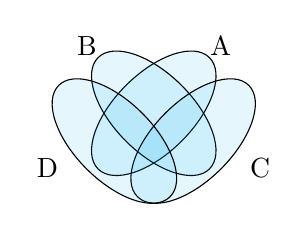
\begin{tikzpicture}[set/.style={fill=cyan,fill opacity=0.1}]
		
		% Ellipse 1 (A)
		\draw[set, rotate=45] (0,0) ellipse (1cm and 0.5cm);
		\node at (0.85,0.85) {A}; % Label for ellipse A
		
		% Ellipse 2 (B)
		\draw[set, rotate=-45] (0,0) ellipse (1cm and 0.5cm);
		\node at (-0.85,0.85) {B}; % Label for ellipse B
		
		% Ellipse 3 (C)
		\draw[set, xshift=0.5cm, yshift=-0.3525cm, rotate=45] (0,0) ellipse (1cm and 0.5cm);
		\node at (1.35,-0.7) {C}; % Label for ellipse C
		
		% Ellipse 4 (D)
		\draw[set, xshift=-0.5cm, yshift=-0.3525cm, rotate=-45] (0,0) ellipse (1cm and 0.5cm);
		\node at (-1.35,-0.7) {D}; % Label for ellipse D
	\end{tikzpicture}

		\subsection*{Basic Definitions}
		\begin{itemize}[leftmargin=*]
			\item Subset: $A \subseteq B \Leftrightarrow \forall x \in A, x \in B$
			\item Not Subset: $A \not\subseteq B \Leftrightarrow \exists x \in A$ s.t. $x \not\in B$
			\item Proper Subset: $A \subsetneq B \Leftrightarrow A \subseteq B \land B \not\subseteq A$
			\item Set Equality: $A = B \Leftrightarrow A \subseteq B \land B \subseteq A$
		\end{itemize}
		\subsection*{Set Operations}
		\begin{itemize}[leftmargin=*]
			\item Union: $x \in X \cup Y \Leftrightarrow x \in X \lor x \in Y$
			\item Intersection: $x \in X \cap Y \Leftrightarrow x \in X \land x \in Y$
			\item Difference: $x \in X - Y \Leftrightarrow x \in X \land x \not\in Y$
			\item Complement: $x \in X^c \Leftrightarrow x \not\in X$
			\item Cartesian Product: $(x,y) \in X \times Y \Leftrightarrow x \in X \land y \in Y$
		\end{itemize}
		\subsection*{Interval Notation}
		\begin{itemize}[leftmargin=*]
			\item $(a,b) = {x \in \mathbb{R} : a < x < b}$
			\item $[a,b) = {x \in \mathbb{R} : a \leq x < b}$
			\item $(a,b] = {x \in \mathbb{R} : a < x \leq b}$
			\item $[a,b] = {x \in \mathbb{R} : a \leq x \leq b}$
			\item $(a,\infty) = {x \in \mathbb{R} : x > a}$
			\item $[a,\infty) = {x \in \mathbb{R} : x \geq a}$
			\item $(-\infty,b) = {x \in \mathbb{R} : x < b}$
			\item $(-\infty,b] = {x \in \mathbb{R} : x \leq b}$
		\end{itemize}
		\subsection*{Special Concepts}
		\begin{itemize}[leftmargin=*]
			\item Disjoint Sets: $A \cap B = \emptyset$
			\item Partition: Sets $A_1, A_2, ...$ where: 1) union is total set and 2) $A_1,A_2,...$ are mutually disjoint
			\item Power Set: $\mathscr{P}(A)$ = set of all subsets
		\end{itemize}
		
		\subsection*{Boolean Algebra Laws}
		note: $0=F=\phi, 1=T=U, + = \lor = \cup,\cdot=\land=\cap,\overline{x}=\neg x = A^c$
		\begin{itemize}[leftmargin=*]
			\item Closure: $\forall a,b\in B, a + b \in B$ and $a \cdot b \in B$
			\item Commutativity: $\forall a,b\in B, a + b = b + a$ and $a\cdot b=b\cdot a$
			\item Associativity: $\forall a,b,c\in B,(a + b) + c = a + (b + c)$ and $(a\cdot b)\cdot c=a\cdot (b\cdot c)$
			\item Distributivity: $\forall a,b,c\in B,a + (b \cdot c) = (a + b) \cdot (a + c)$ and $a\cdot (b+c)=(a\cdot b)+(a\cdot c)$
			\item Identity: $\exists 0,1 \in B, \text{ s.t. }a + 0 = a$ and $a \cdot 1 = a$
			\item Complement: $\forall a\in B, \exists \overline{a}\in B, \text{ s.t. }a + \overline{a} = 1$ and $a \cdot \overline{a} = 0$
			\item Uniqueness of the Complement Law: $\forall a,x \in B$, if $a+x=1$ and $a\cdot x=0$ then $x=\overline{a}$
			\item Uniqueness of 0 and 1: If there exists $x\in B$ such that $\forall a \in B, a+x=1$ and $a\cdot x=0$ then $x=\overline{a}$
			\item Double Complement Law: $\forall a\in B, \overline{(\overline{a})}=a.$
			\item Idempotent Law: $a+a=a$ and $a\cdot a=a$
			\item Universal Bound Law: $a+1=1$ and $a\cdot 0=0$
			\item De Morgan's Laws: $\overline{a+b}=\overline{a}\cdot\overline{b}$ and $\overline{a\cdot b}=\overline{a}+\overline{b}$
			\item Absorption Laws: $(a+b)\cdot a=a$ and $(a\cdot b)+a=a$
			\item Complements of 0 and 1: $\overline{0}=1$ and $\overline{1}=0$.
		\end{itemize}
		
		\subsection*{Russell's Paradox}
		 (e.g. barber who shaves all people who don't shave themselves)
		\begin{itemize}[leftmargin=*]
			\item $S = \{A : A \text{ is a set}, A \notin A\}$
			\item If $S \in S$ then $S \notin S$
			\item If $S \notin S$ then $S \in S$
			\item Resolution: Sets defined within \textit{known} domain
		\end{itemize}
		
		\section*{7. Functions}
		
		\subsection*{Basic Definitions}
		\begin{itemize}[leftmargin=*]
			\item Function $f: X \rightarrow Y$
			\item Total: Every input has output
			\item Single-valued: One output per input
			\item Domain: Input set X
			\item Codomain: Output set Y
			\item Range: $f(X) = \{f(x) : x \in X\}$
		\end{itemize}
		
		\subsection*{Special Functions}
		\begin{itemize}[leftmargin=*]
			\item Identity: $I_X:X\rightarrow X$ where $I_X(a)=a$ for all $a\in X$
			\item Image of a set $A$: $f(A) = \{f(x) : x \in A\}$
			\item Preimage: $f^{-1}(y) = \{x : f(x) = y\}$
			\item Preimage of set: $f^{-1}(A) = \{x\in X : f(x) \in A\}$
		\end{itemize}
		
		\subsection*{Function Properties}
		\begin{itemize}[leftmargin=*]
			\item Injective (1-1):  $f(x)=f(y)\Leftrightarrow x=y$
			\item Surjective (onto): $\forall y \in Y, \exists x: f(x) = y$
			\item Bijective: Both injective and surjective
			\item If a function is bijective (is a bijection), then its inverse is also a function (as opposed to a general relation).
		\end{itemize}
		
		\subsection*{Logarithm Properties}
		\begin{itemize}[leftmargin=*]
			\item $\log_b(xy) = \log_b(x) + \log_b(y)$
			\item $\log_b(\frac{x}{y}) = \log_b(x) - \log_b(y)$
			\item $\log_b(x^y) = y\log_b(x)$
			\item $\log_c(x) = \frac{\log_b(x)}{\log_b(c)}$
		\end{itemize}
		\section*{Algorithm Correctness}
		
		\subsection*{Basic Concepts}
		\begin{itemize}[leftmargin=*]
			\item \textbf{Pre-condition:} Predicate over input values describing valid initial states
			\item \textbf{Post-condition:} Predicate over output values describing required final states
			\item Algorithm is correct if true pre-condition implies true post-condition
		\end{itemize}
		
		\subsection*{Loop Properties}
		\begin{itemize}[leftmargin=*]
			\item Loop is correct iff:
			\begin{itemize}
				\item Pre-condition satisfied
				\item Loop terminates in finite steps
				\item Post-condition satisfied
			\end{itemize}
			\item \textbf{Loop Invariant:}  is a predicate whose domain consists of integers with the following property: if the
			predicate is true at before an iteration, then it is true after the iteration as well. If the following additional
			properties hold, then the loop is correct with respect to its pre- and post-conditions:
			\begin{itemize}
				\item predicate is true before 1st iteration
				\item if the loop terminates after a finite number of iterations, then the truth of the invariant ensures the truth of the post-condition
			\end{itemize}
		\end{itemize}
		
		\subsection*{Loop Invariant Theorem}Given a while-loop with guard G along with its pre- and post-conditions and
		its loop invariant I(n). If all of the following are true, then the loop is correct with respect to its pre- and
		post-conditions.
		\begin{enumerate}[leftmargin=*]
			\item \textbf{Basis property:} pre-condition ensures that $I(0)$ is true.
			\item \textbf{Inductive Property:} for all integers $ k \geq 0$, if the guard $G$ and loop invariant $I(k)$ are both true at the start of an iteration, then $I(k + 1)$ is true at the end of the iteration.
			\item \textbf{Eventual Falsity of Guard:} G becomes false in finite steps
			\item \textbf{Post-condition:} If $N$ is the least number of iterations after which the guard $G$ is false and the loop invariant $I(N)$ is treu, then the post-condition is true.
		\end{enumerate}
	\end{multicols*}
\end{document}